\chapter{A WEB APPLICATION FOR QUICK EXTRACTION AND ANALYSIS OF ARGO DATA}
\label{chap:argo}

\section{Introduction}

Advances in communication and sensor technologies cause the amount of data generated by the Argo program to explode. Sampling the oceans at high resolution creates a data storage problem. Figure~\ref{fig:prof_vs_time} shows the increase as the program continues. The additional data included in each profile due to the Iridium floats compounds each profile size, begging the question as to how can this large data set is accessed. Creating gridded products, inferencing, displaying results becomes an increasingly complex issue as Argo grows in both profile payload and quantity. The web app Argovis is an attempt to address big data in climate science.

\begin{figure}[ht]
\centering
\begin{minipage}{6in}
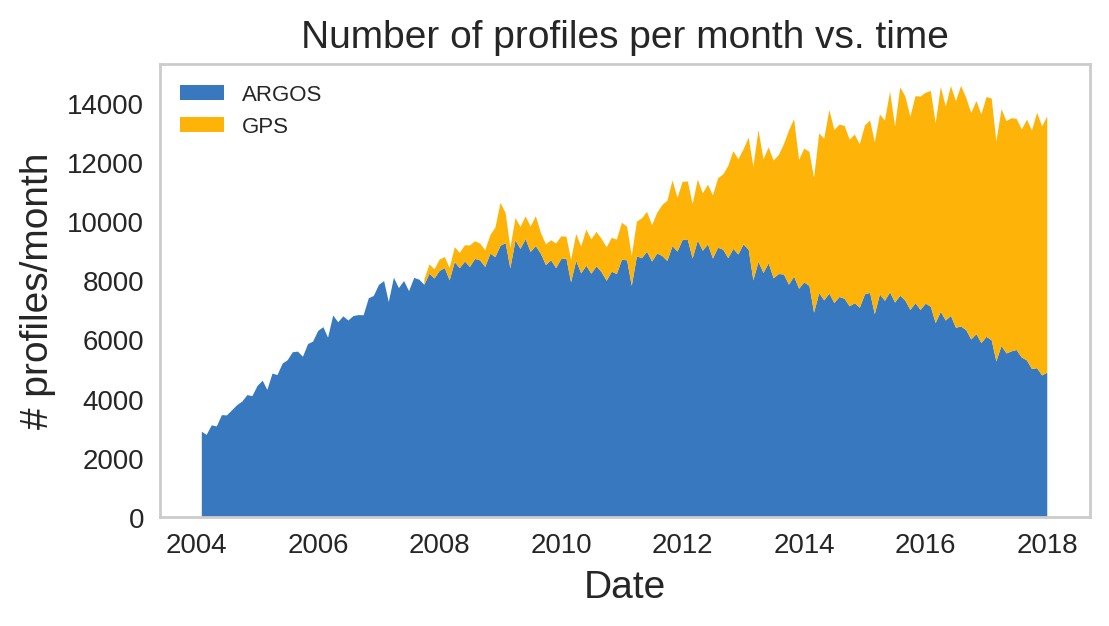
\includegraphics[width=\linewidth]{posSysTypeTS.png}
\caption{\label{fig:prof_vs_time} History of Argo profiles reported each month since the programs inception. Trends towards GPS measurements indicate a need for a data retrival service. Argo data generation is increasing in the number of profiles reported and by the amount of data reported by each profile.}
\end{minipage}
\end{figure}

Data is normally stored in a \gls{gdac} \gls{ftp} server, either at a US-based server at \url{ftp://usgodae.org/pub/outgoing/argo/} or a Europian server at \url{ftp://ftp.ifremer.fr/ifremer/argo/}. The data is assumed to be sufficiently quality controlled and in a stable format. Platform and profile name is the only identification. This data structure does not allow seasonal selection or spatial selection: a key feature to any climate data set. The FTP server is meant to act as an archive. Scientists are encouraged to download the data locally for their uses, a process that relies on significant domain knowledge of the FTP site. Few people will go through the trouble of understanding the FTP structure, and fewer still will take time to make the process easier for others. The current unwieldy system, Stunts the Argo community from expanding.

The Argo program depends on government and by extension, public support. Without the understanding of these parties, the program is in danger of budget cuts, sequestration, and general apathy to scientific endeavor. As is, the public is reliant on the Argo community to extract meaning from the dataset. There is an opportunity to design a system intuitive enough for Laypeople to view data. 

The remainder of this chapter will describe a proposed data storage and visualization system that uses a \gls{dod} to supplant the FTP server, and a RESTfull web app to view database content both spatially and temporally.

\section{Web Application Overview}
The main page, shown in Figure~\ref{fig:main_page}, consists of an interactive map and sidebar with controls, allowing users an intuitive way to navigate through profiles, either a region and date range or by entering a float's WMO number. The map is created using the \gls{leaflet} library.

\begin{figure}[ht]
\begin{minipage}{6in}
\centering
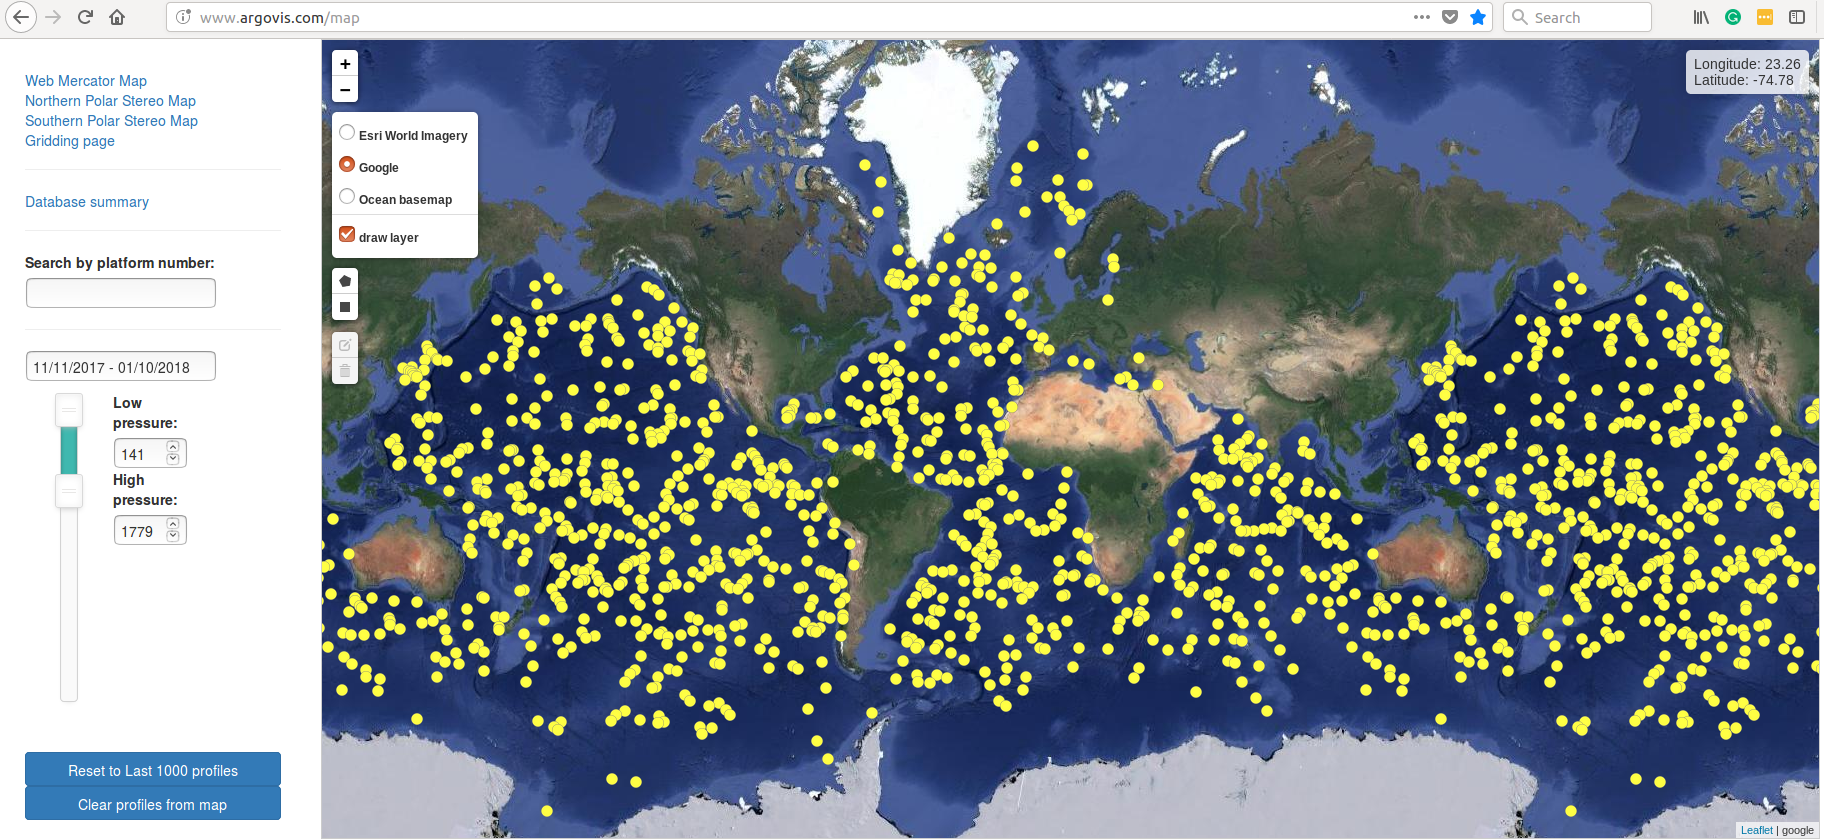
\includegraphics[width=\linewidth]{gEarth.png}
\caption{\label{fig:main_page} Users are greeted by a map with the latest 1000 profiles upon visiting \url{http://www.argovis.com} (top). Clicking on a profile marker springs open a popup window showing additional information and links to its data visualization page. Rectangle and Polygon icons on the map lets the user draw squares or polygons. Upon completion, the map clears all profiles except for the ones that fall within the drawn polygon(s). A pop up over the shape links to another page with T/S/P charts.}
\end{minipage}
\end{figure}
Typing in the known platform name on the side panel reveals the platform's history on the map. Once complete the platform will show up, see Figure~\ref{fig:prof_hist}. Each dot will have a popup window appear when clicked. The window gives lat-lon coordinates, profile's measurement date, a button that will show the float's history. Also included are links to either the platform page, shown in Figure~\ref{fig:profile_data} or the entire float history, shown in Figure~\ref{fig:platform_data}.

\begin{figure}[ht]
\centering
\begin{minipage}{6in}
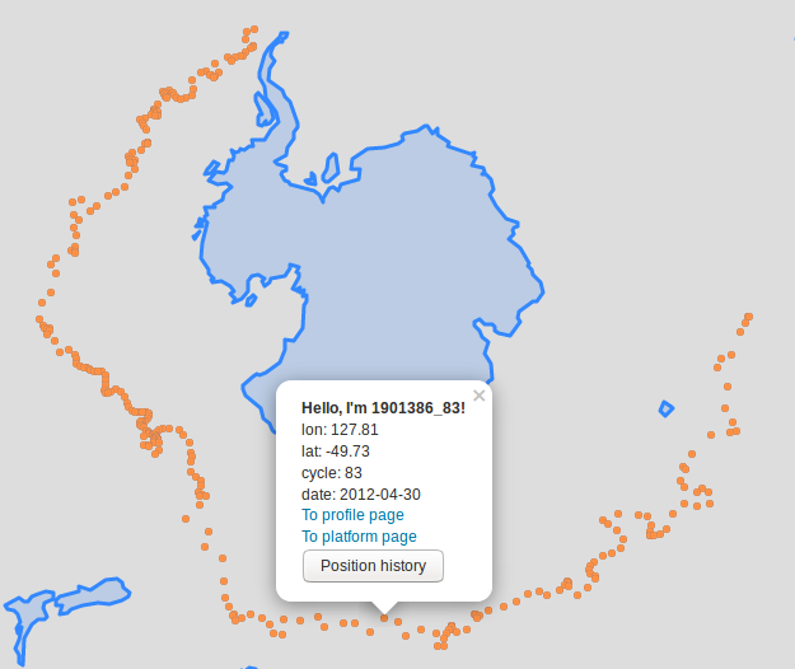
\includegraphics[width=\linewidth]{platformHist.png}
\caption{\label{fig:prof_hist} History of platform 1901386 are shown by orange dots. Each point reprents the float surfacing to transmit its profile information. Clicking on any of the orange profile markes springs open a popup showing additonal information and links to its data visualization page.}
\end{minipage}
\end{figure}

\begin{figure}[ht]
\centering
\begin{minipage}{6in}
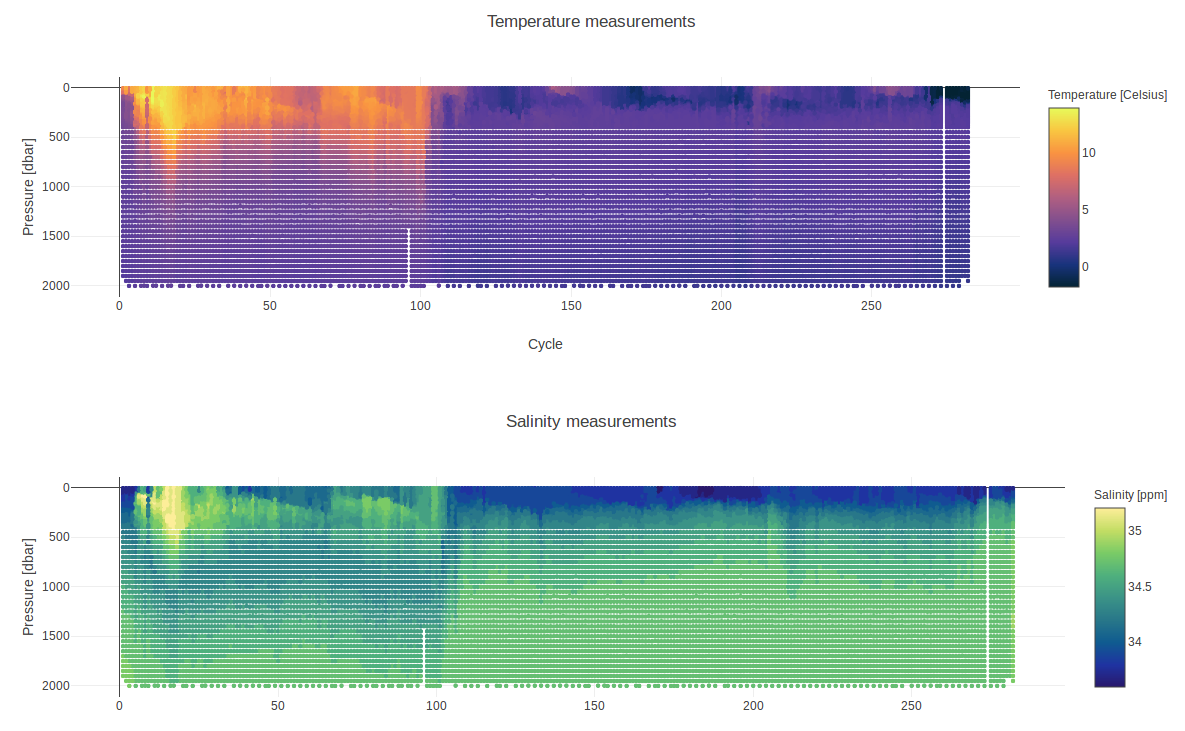
\includegraphics[width=\linewidth]{1901386.png}
\caption{\label{fig:platform_data}Temperature and salinity heat plot for profile 1901386.}
\end{minipage}
\end{figure}

Different map projections are available by clicking the link on the top of the sidebar. Currently, Web Mercator, Northern stereographic, or Southern stereographic are the only web projections available. Only Web Mercator uses map tiles; the latter two use a JSON shapefile to show land outlines. In any projection, the map includes a drawing plugin that allows users to create, edit, and delete squares or polygons. In the event a polygon is created, the app queries the database for profiles falling within the region bounded by the polygon, along with the date and pressure ranges selected on the side panel. If the query isn't too large, the app then clears the map of profiles and returns profiles returned by the database. See Figure~\ref{fig:heart_sel} (top).

The completed shape will also have a popup window show with two buttons that open a page of the selection's T/P/S charts. The same goes for a platform's T/S/P charts can be generated and viewed with a click of a button as shown in Figure~\ref{fig:heart_sel} (bottom).

\begin{figure}[H]
\fbox{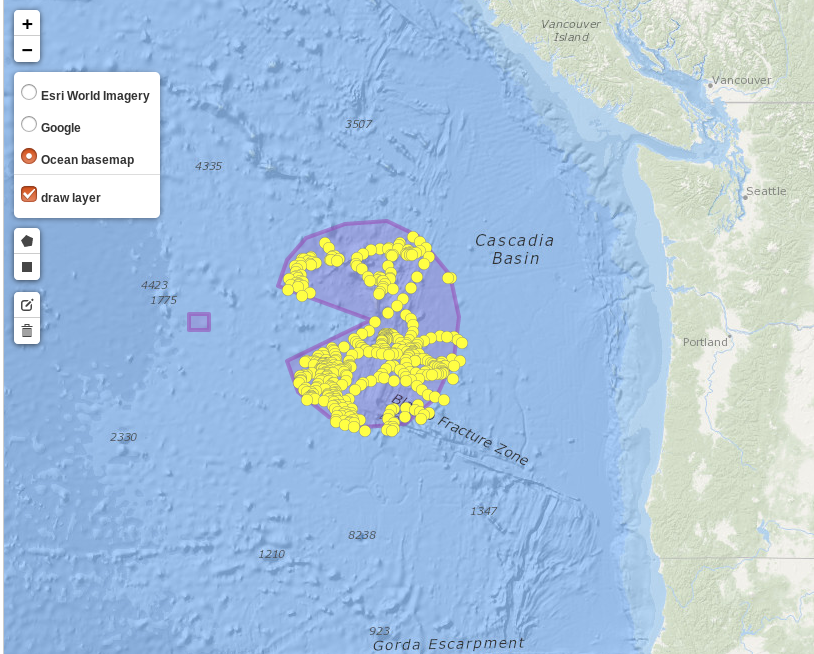
\includegraphics[height=0.22\linewidth]{pacman_map.png}}
\fbox{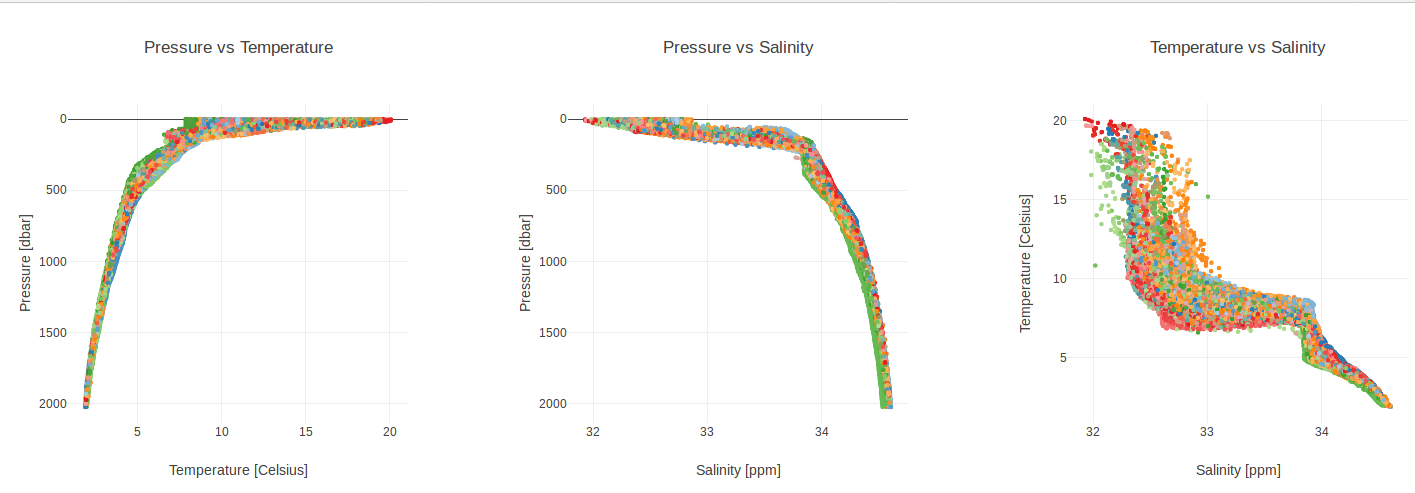
\includegraphics[height=.22\linewidth]{pacmanSelection.png}}
\caption{\label{fig:heart_sel} Upon completion of a shape provided by the drawing tool (top left), the map clears all profiles except for the ones that fall within the drawn polygon(s). A pop up over the shape links to another page with T/S/P charts (mid left). The sidebar includes Date and pressure (depth) range options too.}
\end{figure}

Bottom of page, shown by Figure~\ref{fig:pacman_table} includes a download button, a table, and a table export feature. The page is accessed with the url: \url{http://www.argovis.com/selection/profiles/page?startDate=2010-11-29&endDate=2018-01-28&shape=[[[-132.601318,46.286224],[-130.557861,45.767523],[-132.403564,45.135555],[-132.161865,44.653024],[-131.480712,44.260937],[-130.711669,44.103365],[-129.810791,44.150681],[-129.129638,44.559163],[-128.73413,45.182037],[-128.624267,45.813486],[-128.822021,46.452997],[-129.525146,47.040182],[-130.206298,47.26432],[-131.12915,47.219568],[-131.986084,47.010226],[-132.403564,46.679594],[-132.601318,46.286224]]]}

\begin{figure}[H]
\begin{minipage}{6in}
\centering
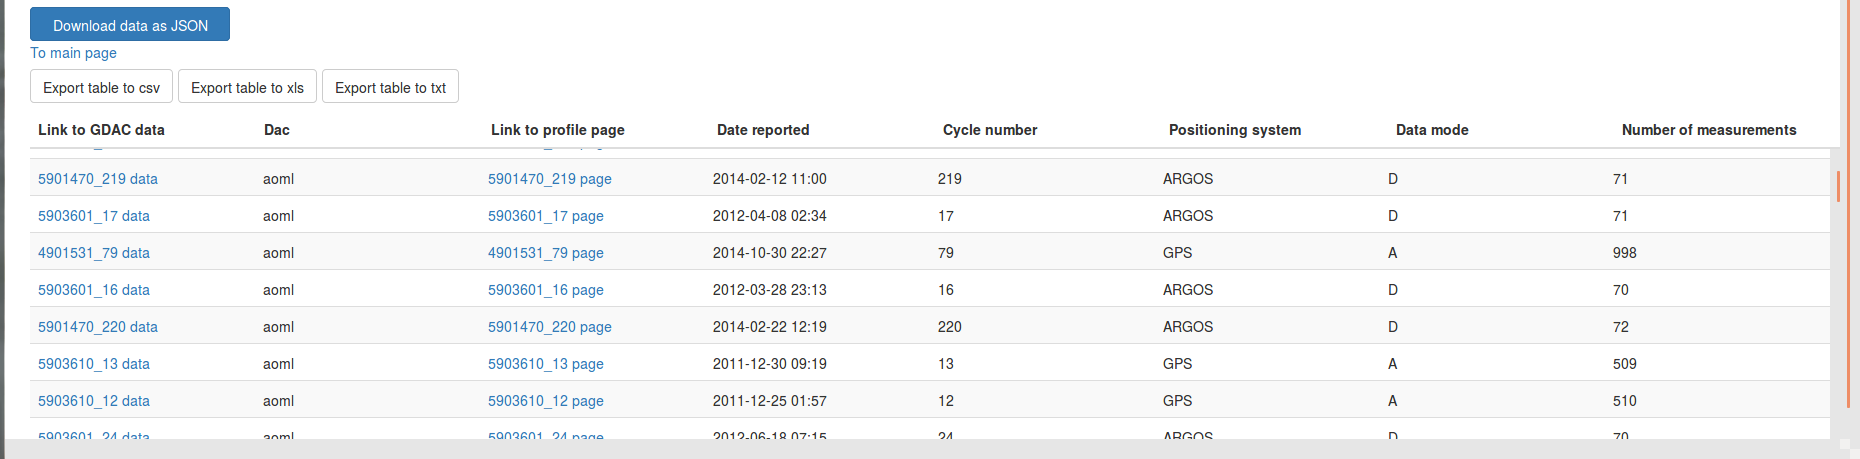
\includegraphics[width=\linewidth]{pacman_table.png}
\caption{\label{fig:pacman_table}Temperature and salinity heat plot for profile 1901386.}
\end{minipage}
\end{figure}

RESTful applications allow clients (either users or other apps) to interact with a database through the URL. In the case of Argovis, users query a MongoDB database filled with ARGO profiles. Users input a set of latitude-longitude coordinates, date range, and pressure range. The Argovis app sends a response: either raw JSON or HTML page with the profile measurements and metadata that fall within these queries. See Figure~\ref{fig:profile_data}. Clients can either download the data directly on their files by clicking the 'Download Data as JSON' button, or by removing from the URL, '/page.' Both profile or selection data is be accessed the same way.

\begin{figure}[H]
\begin{minipage}{6in}
\centering
\fbox{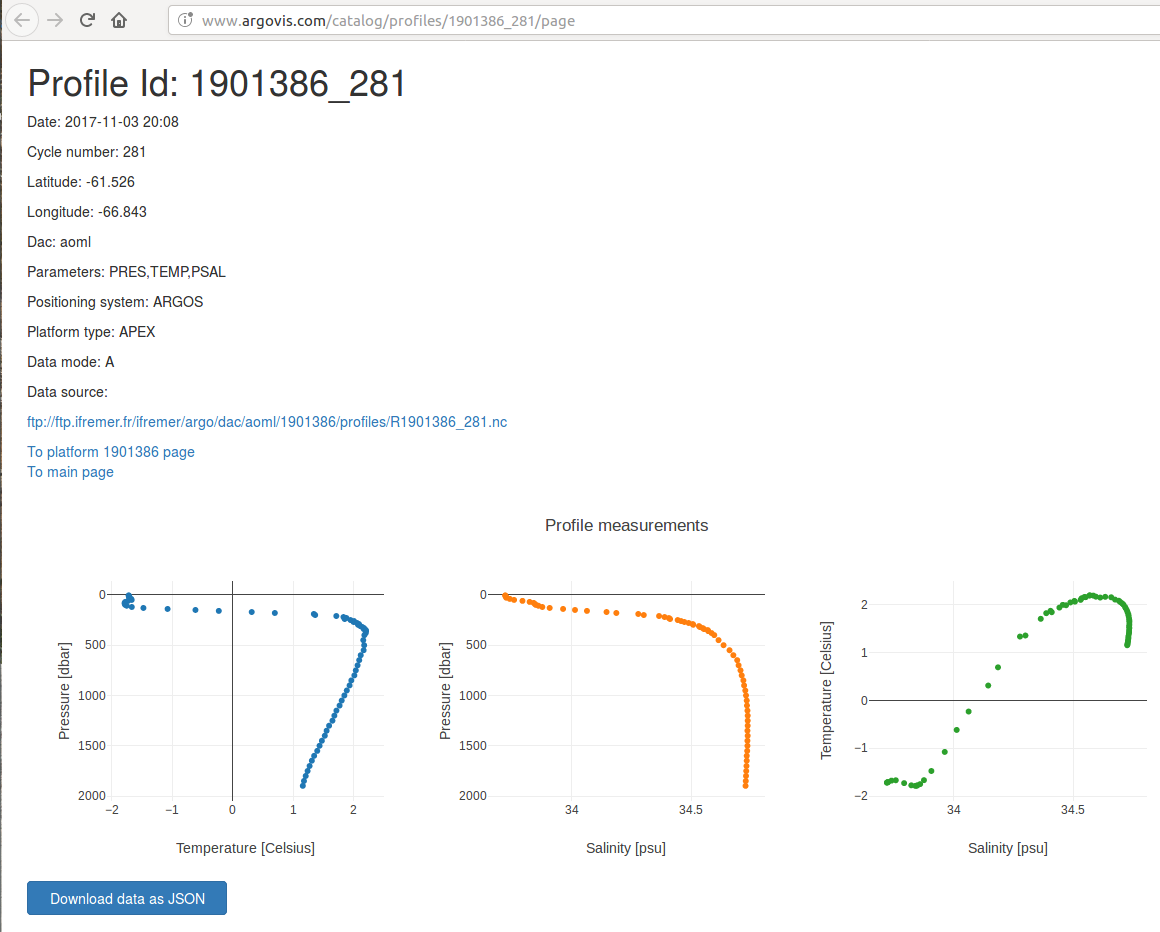
\includegraphics[height=0.39\linewidth]{profilePage.png}}
\fbox{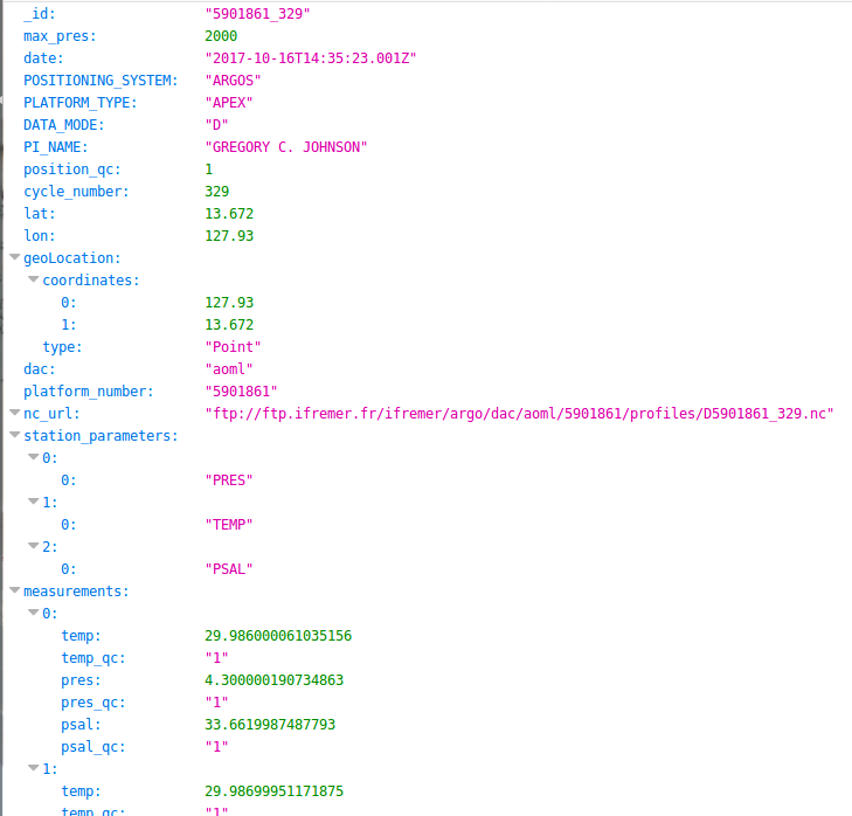
\includegraphics[height=0.39\linewidth]{profileJSON.png}}
\caption{\label{fig:profile_data} Profile page (left), and JSON (right) can be accessed by appending '/page' to the URL (\url{http://www.argovis.com/catalog/profiles/5901861_329/page}) or omitting it.}
\end{minipage}
\end{figure}

\section{Argovis Data Visualization and Extraction Tutorials}

Tutorials describe several website use cases step by step and offers the user a break from reading. The first tutorial narrates a typical use case on how a user can make a custom selection around the Labrador sea at 500-1000 meters during Summer 2017, and download the data and its metadata table locally. The second tutorial has a user track a particular profile over time, view its profiles, examine unusually cold sea surface temperatures, and download a profile directly from the IFREMER GDAC. More data selection and delivery methods are available using the API, covered in Section~\ref{sec:api}. \url{www.itsonlyamodel.us} has more tutorials.

\subsection{Labrador Sea Summer Selection}

This tutorial describes how to make selections on the main page. First, a shape is drawn, followed by a date pressure range. The profiles are viewed and downloaded on a separate page.

\begin{enumerate}
\item Visit \url{www.argovis.com}. You will be greeted by a Web Mercator projection showing profiles reported by the DACS from the past seven days. See Figure ~\ref{fig:main_page}. Sidebar includes a map reset button (Figure~\ref{fig:reset_clear_buttons}, which will return the map to its original state. The clear map button will swipes all profile icons off the map.

\begin{figure}[H]
\begin{minipage}{6in}
\centering
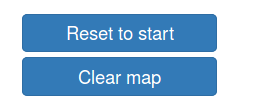
\includegraphics[width=.25\linewidth]{resetClearButtons.png}
\caption{\label{fig:reset_clear_buttons} Reset buttons will return the map to how it was when first rendered by the browser. Clear will remove all profile dots and shapes from the page.}
\end{minipage}
\end{figure}

\item Zoom into the Labrador sea, east of Greenland. You can zoom in by using the mouse wheel or by clicking the zoom button on the top left corner of the map (Figure~\ref{fig:map_draw}

\begin{figure}[H]
\begin{minipage}{6in}
\centering
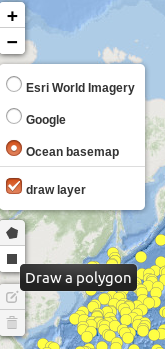
\includegraphics[width=.25\linewidth]{mapDraw.png}
\caption{\label{fig:map_draw} Zoom button (top element) allows zooming in and out. Tile map overlay (2nd down from top) allows the user to choose which map overlay is shown. Rectangle and polygon buttons (3rd down from top) and edit/delete buttons (bottom) lets users draw shaps on the map.}
\end{minipage}
\end{figure}

\item Click the polygon button, located below the zoom buttons and map tile layers on the top left corner of the map.

\item Create a polygon by clicking on the region around the general outline of the Labrador Sea. Circle the polygon nodes back to the point of origin to complete the shape. Upon completion, profiles will only show within the polygon, and a popup will appear (Figure~\ref{fig:lab_sea}. With the shape selected, we next need to specify a date and pressure range.

\begin{figure}[H]
\begin{minipage}{6in}
\centering
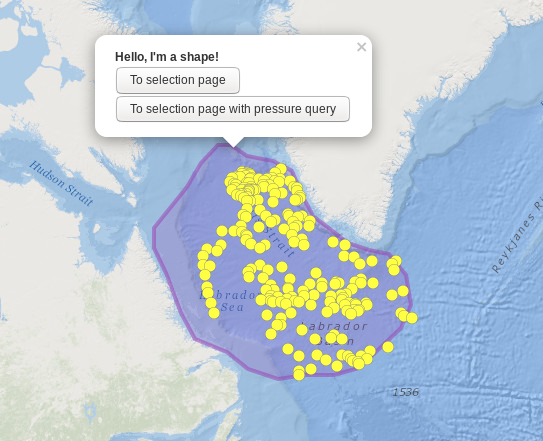
\includegraphics[height=0.39\linewidth]{labSeaMap.png}
\caption{\label{fig:lab_sea} Shape is drawn by pointing and clicking. Complete the shape to query the database and plot profiles. Editing the shape will replot the points with the updated information.}
\end{minipage}
\end{figure}

\item Click on the date input element located on the sidebar. A date range window (Figure~\ref{fig:calender}) will appear comprised of three columns. The left column is an array of buttons with relative times that users can select. The center and right columns display an interactive scrollable calendar that allows for date selections.

\begin{figure}[H]
\begin{minipage}{6in}
\centering
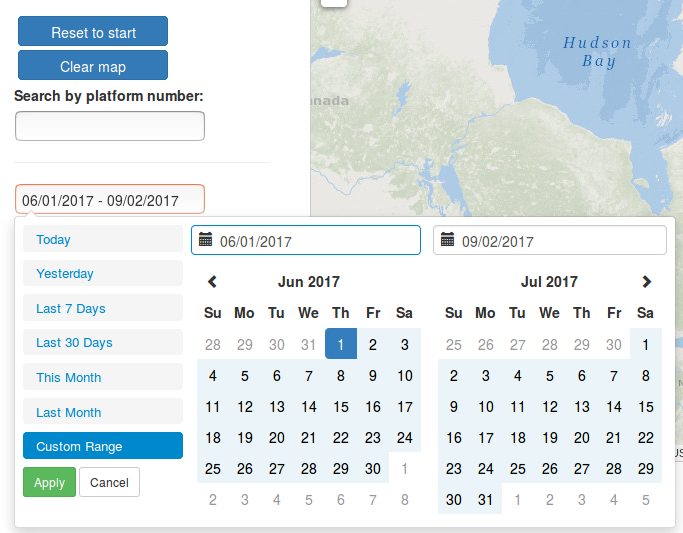
\includegraphics[height=0.39\linewidth]{calender.png}
\caption{\label{fig:calender} Calender feature allows users to select common date ranges (left), click interactively in ranges by clicking days on calender, or by manually typing in date ranges (top textboxes). Upon completion, map is updated. }
\end{minipage}
\end{figure}

\item Adjust the pressure range, located on the sidebar (Figure~\ref{fig:pres_bar}, so that the upper pressure is at 1000 dbar and the lower pressure is at 500 dbar. You can either adjust the double scroll bar using the mouse, click the arrows located in the input element. You may also type in the number of input element directly followed by pressing enter. Each time pressure is adjusted updates the profiles in the polygon area.

\begin{figure}[H]
\begin{minipage}{6in}
\centering
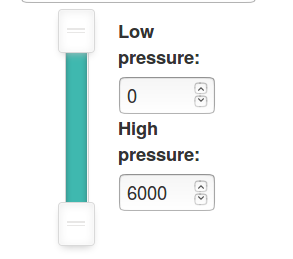
\includegraphics[height=0.25\linewidth]{presBar.png}
\caption{\label{fig:pres_bar} Pressure slider bar contains two sliders that set upper and lower pressure ranges. Upon a change, the map is updated. Text boxes are syncronized to slider bar such that any changes are updated on all three elements.}
\end{minipage}
\end{figure}

\item Open the selection page by clicking on the shape popup button labeled "To selection page with pressure query. This page (Figure~\ref{fig:lab_sel_page} can be viewed through the \url{http://www.argovis.com/selection/profiles/page?presRange=[500,1000]&startDate=2017-06-01&endDate=2017-09-02&shape=[[[-54.8291,53.696706],[-56.674803,54.572062],[-59.487303,55.229023],[-60.717772,56.511018],[-62.036131,58.401712],[-63.090819,59.534318],[-63.090819,60.413852],[-61.508787,61.312452],[-60.190428,62.144976],[-58.959959,63.114638],[-57.465819,63.821288],[-56.32324,63.821288],[-54.91699,63.391522],[-52.631834,63.194018],[-50.961912,62.794935],[-49.995115,61.731526],[-49.116209,60.930432],[-47.79785,60.457218],[-46.040037,59.756395],[-44.194334,59.445075],[-42.436522,59.265881],[-40.942381,58.309489],[-40.502928,56.897004],[-41.381834,55.776573],[-42.788084,55.028022],[-45.07324,53.748711],[-47.270506,53.383328],[-49.731444,53.383328],[-52.192381,53.173119],[-54.8291,53.696706]]]}.

%\url{http://www.argovis.com/selection/profiles/page?presRange=[500,1000]&startDate=2017-06-01&endDate=2017-09-02&shape=[[[-54.8291,53.696706],[-56.674803,54.572062],[-59.487303,55.229023],[-60.717772,56.511018],[-62.036131,58.401712],[-63.090819,59.534318],[-63.090819,60.413852],[-61.508787,61.312452],[-60.190428,62.144976],[-58.959959,63.114638],[-57.465819,63.821288],[-56.32324,63.821288],[-54.91699,63.391522],[-52.631834,63.194018],[-50.961912,62.794935],[-49.995115,61.731526],[-49.116209,60.930432],[-47.79785,60.457218],[-46.040037,59.756395],[-44.194334,59.445075],[-42.436522,59.265881],[-40.942381,58.309489],[-40.502928,56.897004],[-41.381834,55.776573],[-42.788084,55.028022],[-45.07324,53.748711],[-47.270506,53.383328],[-49.731444,53.383328],[-52.192381,53.173119],[-54.8291,53.696706]]]}.

\begin{figure}[H]
\begin{minipage}{6in}
\centering
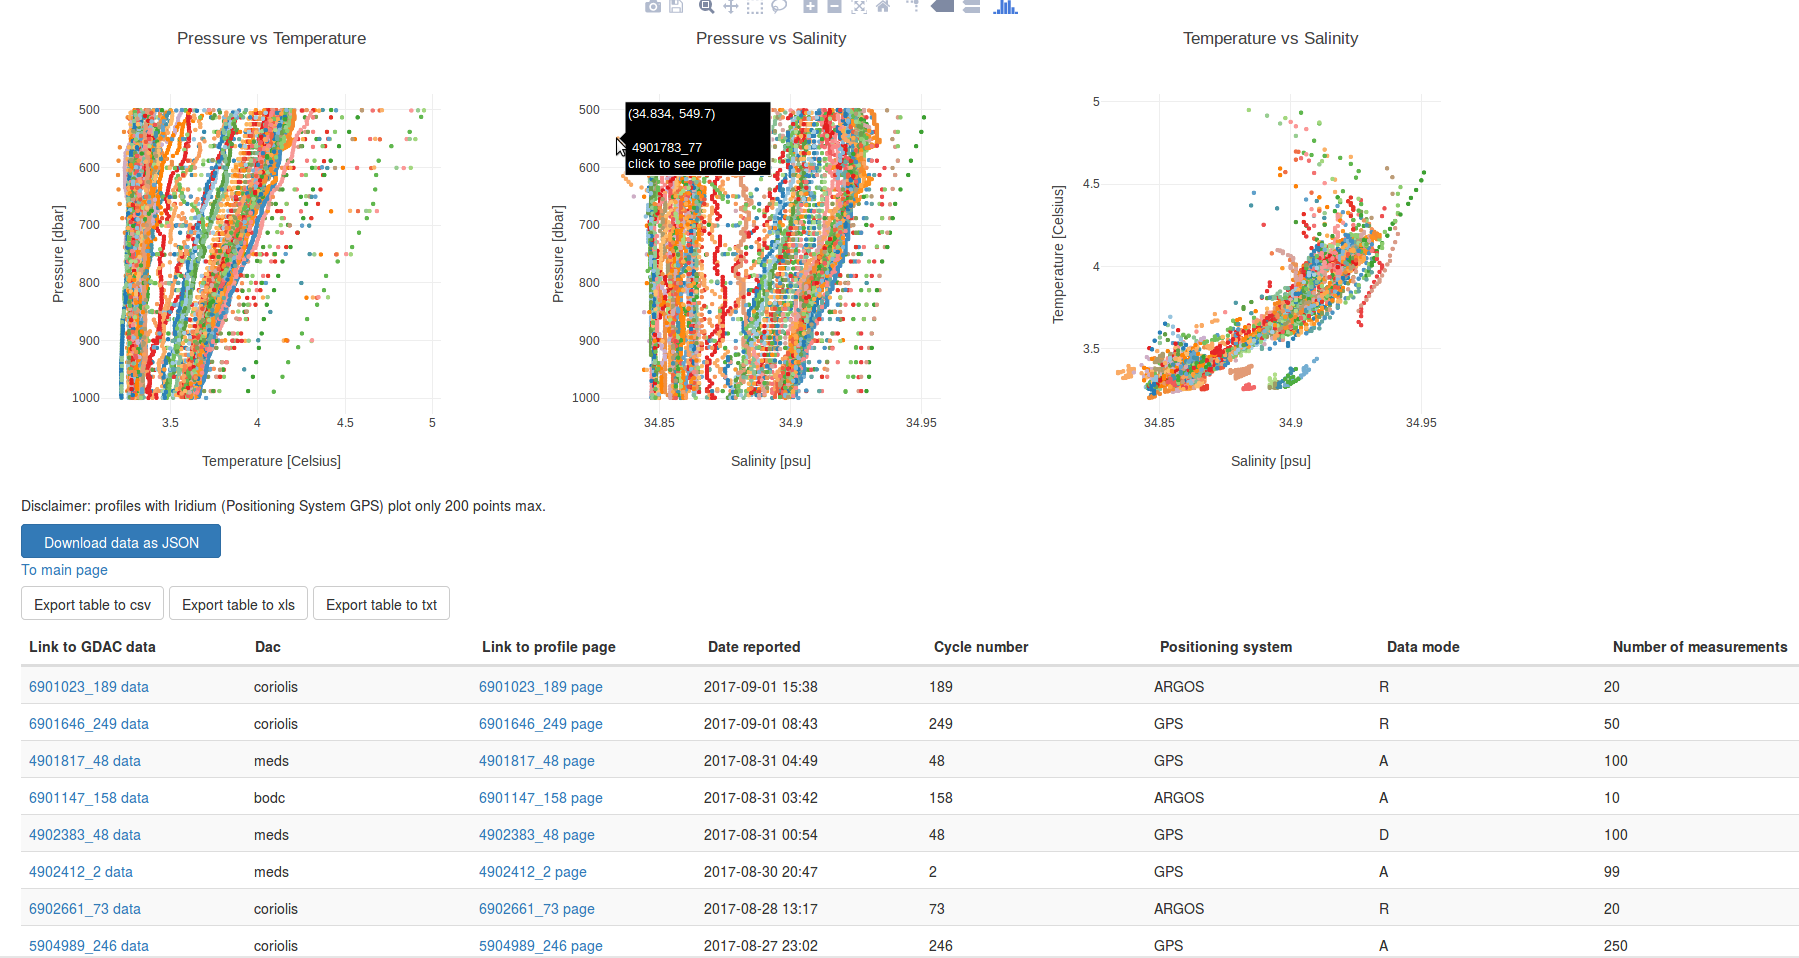
\includegraphics[width=\linewidth]{labSelPage.png}
\caption{\label{fig:lab_sel_page} Selection page is comprised of T/S/P plots (top). Each color represents a profile. Hovering the cursor over will reveal a popup that displays position coordinates and profile id. Clicking on a point will open the profile page in another link. "Download data as JSON" button opens JSON file containing selection data in a separate window. "To main page" link sends the user back to home page. Export buttons allow users to download the table of profile metadata shown below. A table includes links to download profiles directly from the GDAC.}
\end{minipage}
\end{figure}

The T/S/P plots showing selection data is instantly available for view. Each color represents a single profile. Hovering the cursor shows the detail. Clicking on while the cursor is hovering over a profile will open the page for that particular profile. 

\item Download the raw data by clicking on the "Download Data" button. A new tab on the browser will open, showing the data in a JSON format.

\item Download the table of profile Metadata as a .csv file by clicking on the "Download as csv" button. Excel spreadsheet or text format is also available.

\end{enumerate}

You should now have as much data as the database for this section locally. 

\subsection{Track a single platform in the Southern Ocean}

This tutorial shows Argovis's ability for a user to track a particular profile over time, view its profiles, examine unusually cold sea surface temperatures, and download a profile directly from the IFREMER GDAC.

\begin{enumerate}

\item Visit \url{www.argovis.com}. You are greeted by a Web Mercator projection showing profiles reported by the DACS from the past seven days.

\item Click the "Southern Polar Stereo Projection" button that redirects you to a new page with a map that uses a Southern polar stereographic projection (Figure~\ref{fig:south_map}.

\begin{figure}[H]
\begin{minipage}{6in}
\centering
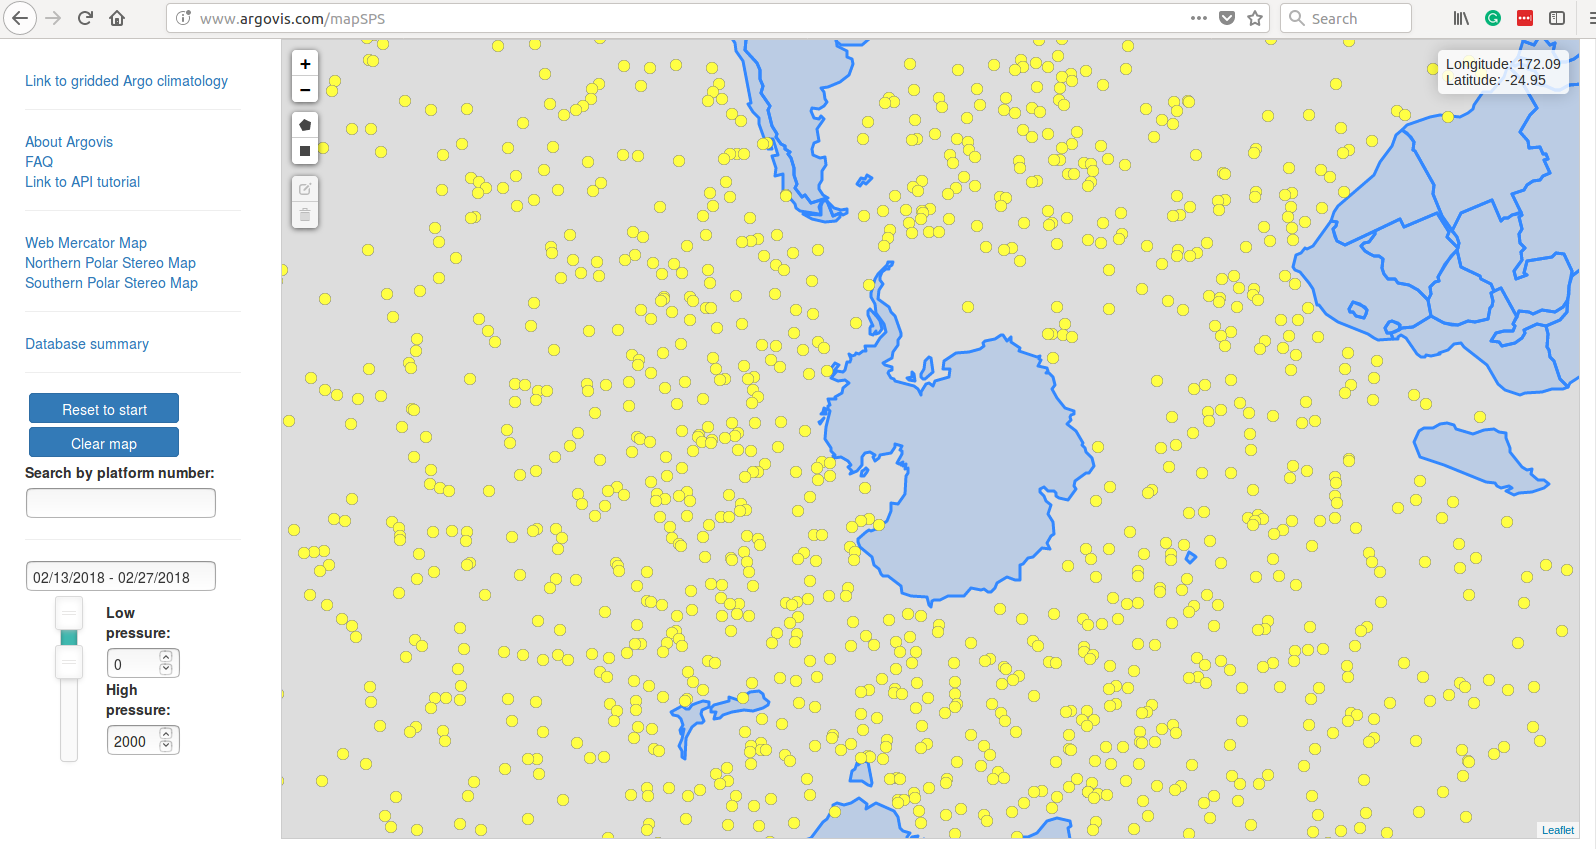
\includegraphics[width=\linewidth]{southSeaMap.png}
\caption{\label{fig:south_map} Southern Stereographic projection map view. Map tile layers are not available under this projection. Land is displayed using geoJSON shape files.}
\end{minipage}
\end{figure}

\item Clear the map by clicking the "Clear Map" button located the sidebar.

\item Enter the WMO/platform number 1901386 in the "Search by platform number" textbox. The profiles generated by this platform will be displayed circling Antartica (Figure~\ref{fig:1901386}).

\begin{figure}[H]
\begin{minipage}{6in}
\centering
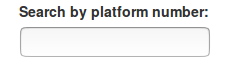
\includegraphics[width=.3\linewidth]{searchByPlatform.png}
\caption{\label{fig:platform_search} "Search by platform number" textbox will plot a platform's profiles on the map. Profiles are displayed in orange. Profiles are displayed when the user enters in a profile number. Four characters or more is enough to query the database. }
\end{minipage}
\end{figure}

\begin{figure}[H]
\begin{minipage}{6in}
\centering
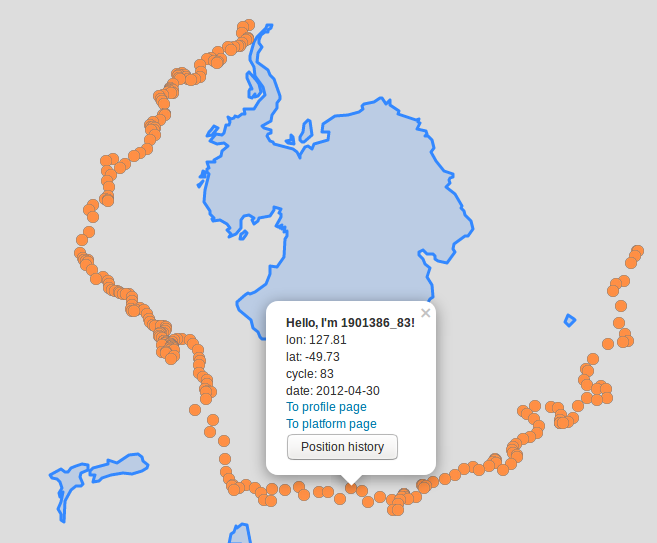
\includegraphics[width=.75\linewidth]{profTrackingSouthSter.png}
\caption{\label{fig:1901386} Profiles that are plotted using platform selection button appear in Orange. Clicking on any point will bring up a popup icon with the profiles id, position, cycle number, and date. Also included are links to the profile's page and its platform page. Position history button will display the other profiles of the same platform.}
\end{minipage}
\end{figure}

\item Click on any orange point to bring up a profile popup window. Click the "To platform page" link to open up the page in another browser tab (Figure~\ref{fig:colorPlots}). The page resides at \url{http://www.argovis.com/catalog/platforms/1901386/page}.

\begin{figure}[H]
\begin{minipage}{6in}
\centering
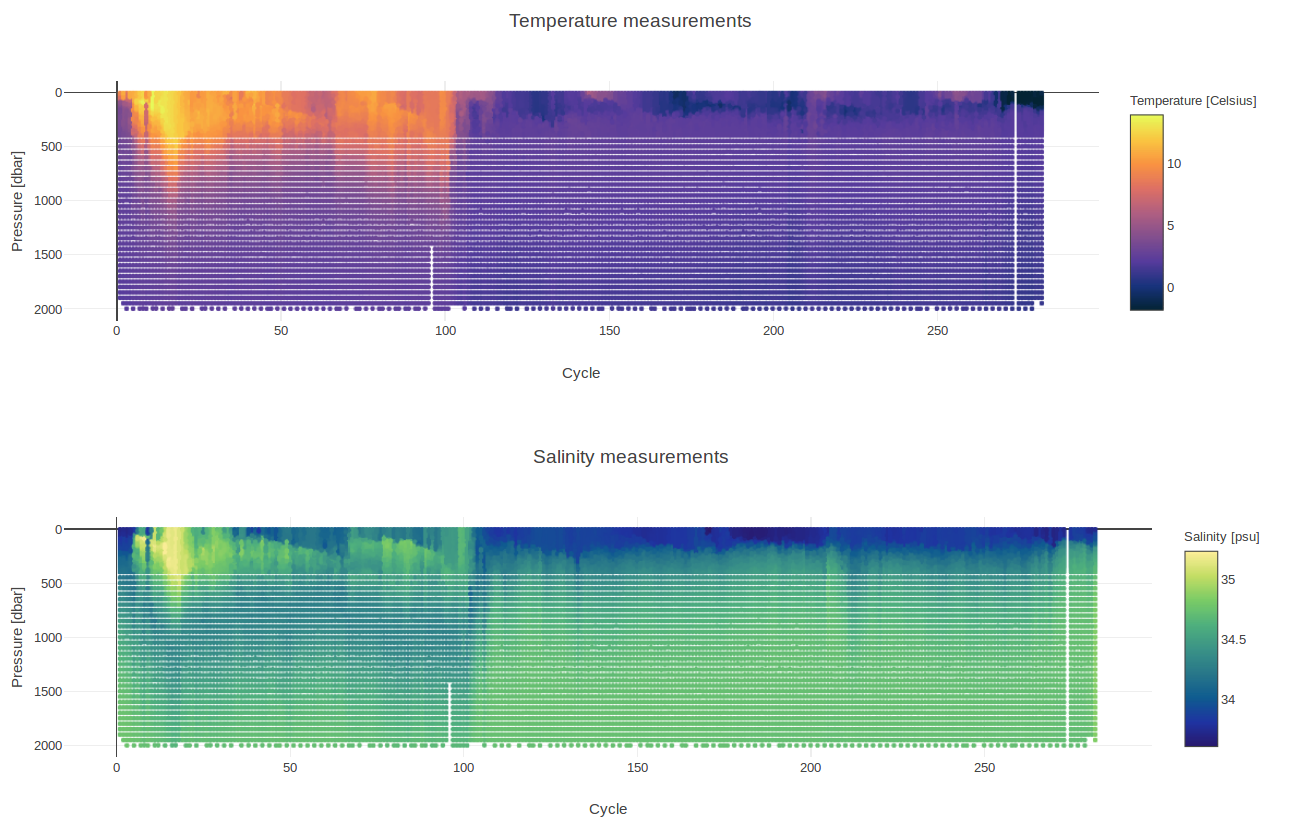
\includegraphics[width=\linewidth]{colorPlots.png}
\caption{\label{fig:colorPlots} Profiles of the same platform are plotted with color charts. The platform page shows temperature (top) and Salinity (bottom). The vertical axis represents pressure (depth), and the horizontal is cycle number. Like the selection page, hovering the cursor over any point will trigger a popup with the values of the point. Clicking on the point will open the profile's page.}
\end{minipage}
\end{figure}

Color plot of shows temperature going unusually low at the surface. Negative temperatures may be an error and will be investigated as an exercise.

\item Click on the dark purple region in the upper right corner of temperature color plot. In this case. A new browser tab will open, showing the profile page you just clicked. In this example, profile $1901386$\textunderscore$281$ was selected and is shown in Figure~\ref{fig:profilePage}. This page resides at \url{http://www.argovis.com/catalog/profiles/1901386_281/page}.

\begin{figure}[H]
\begin{minipage}{6in}
\centering
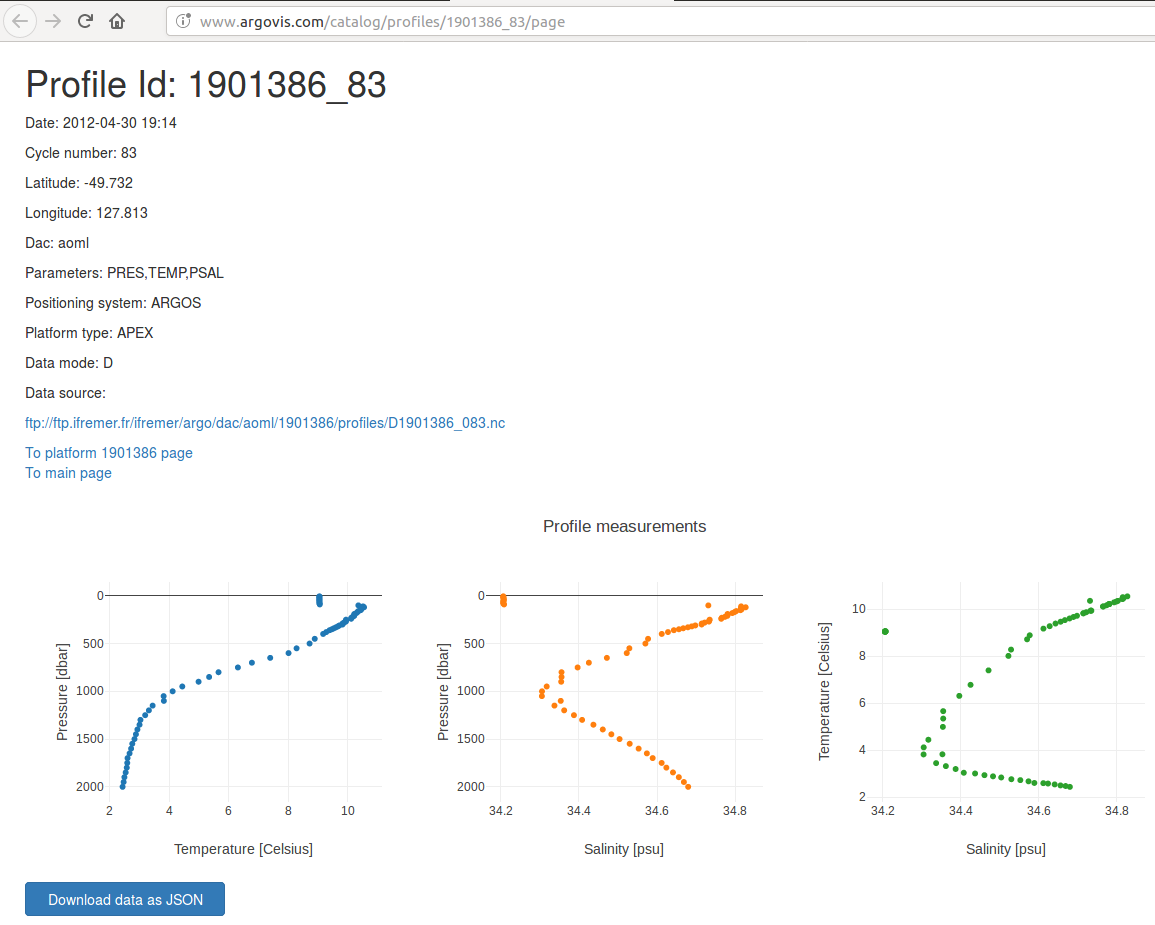
\includegraphics[width=\linewidth]{profPage.png}
\caption{\label{fig:profilePage} Platform page of id $1901386$\textunderscore$281$. Meta information is displayed first. Data source links to the original netCDF file located at the GDAC. There are also links that will direct the user back to the platform page or main page. T/S/P charts are on the bottom. Data used to generate the page can be downloaded by clicking the "Download data as JSON" button.}
\end{minipage}
\end{figure}

The date this profile surfaced was on November 3rd, 2017. Ice sheets melt, making the surface temperatures cold and brackish. Salinity is around 34 \gls{psu}. The profile location is close to the Antartic peninsula, indicating that the ice sheets connected to the land are relatively close. Most likely, this data is accurate. As it turns out, sea temperatures freeze at about -2 Celsius \cite{noaaOcean}. To make sure that the reported data matches the original netCDF file reported in the GDAC the profile page includes a link that will download the netCDF file when clicked. 

\item Click on the link \url{ftp://ftp.ifremer.fr/ifremer/argo/dac/aoml/1901386/profiles/R1901386_281.nc} to download this profile data directly from the ifremer GDAC. You now have the original data opened with software compatible with netCDF files to compare to the unusually low sea surface temperatures. 

\end{enumerate}

\subsection{Value added educational tool: Argovis video tutorials}

Video tutorials are included on \url{https://www.youtube.com/playlist?list=PLJQE6R74BkyVV3PeTRdGh-W5llAY4XJ8v}. The videos guide users through a series of Argovis's features. The advantage of videos over paper tutorials is that users can view, pause, and rewind videos. Youtube also broadcasts the videos over their website, increasing the odds of new users stumbling upon the app. Youtube videos also provide feedback input. The user community can voice support, frustrations, requests in this medium.  Figure~\ref{fig:yt-vids} shows a screenshot of the videos released at the time this thesis was written.

\begin{figure}[H]
\begin{minipage}{6in}
\centering
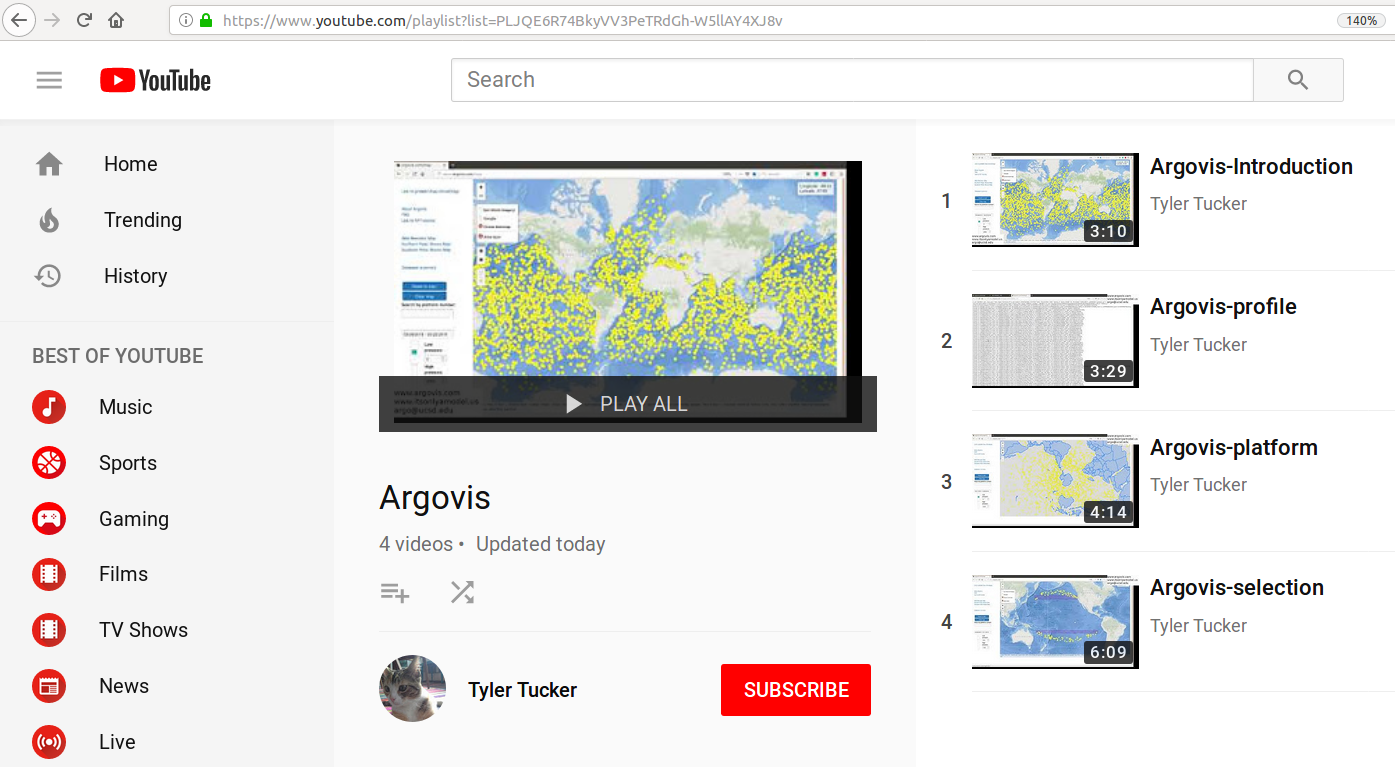
\includegraphics[width=\linewidth]{video-tutorials.png}
\caption{\label{fig:yt-vids} Screenshot of Argovis playlists on YouTube \url{https://www.youtube.com/playlist?list=PLJQE6R74BkyVV3PeTRdGh-W5llAY4XJ8v} . }
\end{minipage}
\end{figure}

\section{Back-End Overview}
Argovis uses the \gls{express} framework to host dynamic web pages. The framework handles page views, routing, and database interface. In addition to the base T/S/P parameters, floats may contain $O_2$, $N_2$, Conductivity, et cetera. A \gls{mongodb} database stores the profiles metadata and their measurements as Binary JSON objects. Argo data pairs well with MongoDB's flexible schema. For example, not all profiles have to have a $N_2$ field.

\subsection{Data Format and Delivery}

Profiles are stored as document objects. Each document has a schema as seen in Listing~\ref{lst:label}. The "measurements" field must contain temperature, salinity and pressure, but may also contain fields found on Table~\ref{tbl:argoParams}
\begin{lstlisting}[language=JavaScript, label={lst:label}, caption=JSON schema of mongoDB profile.]
{
  "_id": <String>,
  "max_pres": <Int>,
  "measurements": <List[{temp: <Number>,
                         psal: <Number>,
                         pres: <Number>,
                         ...}]>,
  "date": <ISODate>,
  "POSITIONING_SYSTEM": <String>,
  "PLATFORM_TYPE": <String>,
  "DATA_MODE": <String>,
  "PI_NAME": <String>,
  "cycle_number": <Int>,
  "lat", <Number>,
  "lon", <Number>,
  "geoLocation", {"type": "Point",
                  "coordinates": [<Number[2]>],
  "dac": <String>,
  "platform_number": <String>,
  "station_parameters": <List[String]>, 
  "nc_url": <String>
}
\end{lstlisting}

MongoDB outputs \gls{json} data. JSON format is used to create the map, profile, platform, and selection aspects of the website. API access also uses JSON and will be mentioned in Section~\ref{sec:api}. JSON 'curly braces' encapsulate the Javascript data types. 

\subsection{Database Architecture}

Indexing shrinks the query time significantly. Currently, date, platform\textunderscore number, cycle\textunderscore number, DAC, and geoLocation are indexed.

Each day new profiles are added to the GDAC, and old profiles are updated. Argovis is synchronized with the GDAC daily to reflect new changes, such as introducing new profiles or correcting errors by the GDAC. Each day, a \gls{cron} script runs a shell script that updates a local mirror of the IFREMER GDAC using the \gls{rsync} command. A script of changes is created in the process and fed to a python algorithm that adds or replaces the files that are in the database. The script is found in Appendix~\ref{append:update_db}. 

Transforming netCDF files from the GDAC FTP server involves reformatting the .nc files to the document schema shown in Listing~\ref{lst:label}. The script parses netCDF files and adds portions of its 'variables' field to the database. Additionally, some erroneous data and low quality are removed, as the GDACs keep all data. Each measurement in the Argo program has a \gls{qc} string value, whose meanings are shown in Table~\ref{tbl:qc}. The current version of Argovis includes measurements that have a QC flag of 1.

\begin{table}[th]
\centering
\caption{Argo Quality control flag meanings, taked directly from Argo Manual \cite{argo_man}}
\label{tbl:qc}
{\begin{tabular}{ | p{3cm} | p{5cm} |} 
        \hline
        \textbf{N} & \textbf{Meaning} \tabularnewline \hline
        0 & No QC was performed \tabularnewline \hline
        1 & Good data \tabularnewline \hline
        2 & Probably good data \tabularnewline \hline
        3 & Bad data that is potentially correctible \tabularnewline \hline
        4 & Bad data \tabularnewline \hline
        5 & Value changed \tabularnewline \hline
        8 & Interpolated value \tabularnewline \hline
        9 & Missing value \tabularnewline \hline
        \end{tabular}}
\end{table}

The following pseudocode \ref{alg:ncToDb} outlines the .nc to MongoDB process as a rough outline.

\begin{algorithm}
\caption{profile *.nc files to MongoDB document}\label{alg:ncToDb}
\begin{algorithmic}[1]
\Procedure{Convert file to document}{}
\State $\texttt{Generate lists of profile names for each dac from local GDAC}$
\Loop{\texttt{ each dacList in listOfDacLists}}
\State $\texttt{document} = []$
\Loop{\texttt{ each fileName in dacList}}
\State $\texttt{get pathName from fileName}$
\State $\texttt{get dacName from dacList}$
\State $\texttt{open file, get variables field}$
\State $\texttt{doc} = \texttt{MAKE\textunderscore PROF\textunderscore DOC(variables, pathName, dacName, remotePath)}$
\State $\texttt{append doc to documents}$
\If{\texttt{documents length greater than threshold}}
\State $\texttt{add documents to MongoDB}$
\State $\texttt{document} = []$
\EndIf
\EndLoop
\State $\texttt{add remaining documents to MongoDB}$
\EndLoop
\EndProcedure
\Procedure{make\textunderscore prof\textunderscore doc}{}
\State \textbf{INPUT:} \texttt{variables, pathName, dacName, remotePath}
\State retrieve platformNumber, stationParameters, referenceDate from variables
\State $\texttt{idx}=0$
\State $\texttt{qcThreshold}='1'$
\State $\texttt{p2D} = \texttt{netCDFToDoc(...)}$
\State $\texttt{doc} = \texttt{p2D.get\textunderscore profile\textunderscore doc()}$
\State \textbf{OUTPUT:} \texttt{doc}
\EndProcedure
\end{algorithmic}
\end{algorithm}

MongoDB's database accepts one document or multiple documents at a time, the latter speeds up the algorithm, hence Algorithm~\ref{alg:ncToDb} collects documents in RAM before adding it to MongoDB. Python excels at handling complex data objects. For this reason, it was chosen to implement Algorithm~\ref{alg:ncToDb} and ~\ref{alg:ncToDb}.

The class netCDFToDoc\ref{alg:netCDFToDoc} takes some of netCDF's variables, performs QC, and bundles parameters into a JSON object that MongoDB can accept. In a pythonic context, dictionary types are equivalent to JSON. See Algorithm~\ref{alg:netCDFToDoc}.

\begin{algorithm}
\caption{netCDFToDoc class formats netCDF data into JSON object}\label{alg:netCDFToDoc}
\begin{algorithmic}[1]
\Procedure{create a JSON/dict object}{}
\State \textbf{INPUT:} \texttt{variables, pathName, dacName, remotePath}
\State \textbf{INPUT:} \texttt{platformNumber, stationParameters, referenceDate}
\State $\texttt{init measDataFrame}$
\State $\texttt{measurement = ['temp', 'pres', 'psal', 'cndc', 'doxy', ... ]}$
\Loop{\texttt{ each meas in measurements}}
\State $\texttt{from variables get measArray, measQCArray, adjMeasArray, adjMeasQCArray}$
\Loop{\texttt{ each (value, idx) in measArray}}
\If{\texttt{adjMeasArray[idx] exists}}
\State $\texttt{measArray[idx] = adjMeasArray[idx]}$
\State $\texttt{measQCArray[idx] = adjMeasQCArray[idx]}$
\EndIf
\State $\texttt{combine arrays into singDataFrame}$
\EndLoop
\State $\texttt{drop row in singDataFrame if QC column} \neq 1$
\State $\texttt{concat singDataFrame to measDataFrame (preserving index)}$
\EndLoop
\State $\texttt{replace NaN with -999 in measDataFrame}$
\State $\texttt{drop row in measDataFrame if measDataFrame['pres'] == -999}$
\State $\texttt{drop all qc columns in measDataFrame}$
\State $\texttt{init doc = dict()}$
\State $\texttt{doc['max\textunderscore pres'] = measDataFrame['pres'].max()}$
\State $\texttt{doc['measurements'] = measDataFrame.toList(orient='records')}$
\State $\texttt{doc['date'] = variables['JULD'] - referenceDate}$
\State $\texttt{doc['lat'] = variables['LATITUDE']}$
\State $\texttt{doc['lon'] = variables['LONGITUDE']}$
\State $\texttt{doc['POSITIONING\textunderscore SYSTEM'] = variables['POSITIONING\textunderscore SYSTEM']}$
\State $\texttt{doc['PLATFORM\textunderscore TYPE'] = variables['PLATFORM\textunderscore TYPE']}$
\State $\texttt{doc['DATA\textunderscore MODE'] = variables['DATA\textunderscore MODE']}$
\State $\texttt{doc['PI\textunderscore NAME'] = variables['PI\textunderscore NAME']}$
\State $\texttt{doc['POSITION\textunderscore QC'] = variables['POSITION\textunderscore QC']}$
\State $\texttt{doc['cycle\textunderscore number'] = variables['CYCLE']}$
\State $\texttt{doc['geoLocation'] = dict('type':'Point','coordinates':[lon, lat])}$
\State $\texttt{doc['dac'] = dacName}$
\State $\texttt{doc['platform\textunderscore number'] = platformNumber}$
\State $\texttt{doc['nc\textunderscore url'] = 'ftp://ftp.ifremer.fr/ifremer/argo/dac/'+remotePath}$
\State $\texttt{doc['\textunderscore id'] = platformNumber + variables['CYCLE']}$
\State \textbf{OUTPUT:} \texttt{doc}
\EndProcedure
\end{algorithmic}
\end{algorithm}

Measurements may contain values adjusted by the DACS; however, Argovis will replace the original with the adjusted if it exists(lines 9-11). The netCDFToDoc algorithm filters the data so that only QC = 1 make it to the database (line 13). Measurements are all bundled in one \gls{dataframe} object (line 14). An exception to the rule, rows of this concatenated dataframe are dropped if there are unknown pressure values (line 16); pressure values are needed to generate plots and filter on the front-end side. '-999' replaces missing values.' Finally, the QC columns, no longer needed are dropped. The remaining lines 19-34 add meta information with minimal formatting.

This process is repeated daily for new files using a \gls{cron} script. New/updated profiles are detected and downloaded from the GDAC to a local directory. A list of the profiles is fed to the python script, which runs Algorithms~\ref{alg:netCDFToDoc} and ~\ref{alg:ncToDb}.

\section{Python API}\label{sec:api}

Argovis is designed to be used by both professional and amateur alike. The front end is intuitive but can be confining for automated tasks. Additional visualization features can be added, at the expense of additional development cost and maintainability. Feature creep in web apps complicates an otherwise intuitive design. On the other hand, a sparsely featured application discourages experts/scientists from using the app. \gls{api} services are the balance that reconciles the design conflict between ease of use and visualization features.

The definition of API is somewhat nebulous, but this context an API is access to data without the need of a browser. It is often referred to as "Machines talking to machines" In this case, it is custom code talking to Argovis. The custom code can be a process running a plotting script, a data archive service, or even another website. Scientists can make selections using a script in their preferred language by including HTTP APIs.

One such API has been implemented in Python. A suite of functions listed in the Appendix~\ref{append:python_api} retrieve data from Argovis. All other features for visualization and computing depend on these functions. RESTfully designed apps such as Argovis allow non-browser apps to retrieve data. Accessing Argovis is as simple as writing a few lines using the request library. The different ways to visualize data surpasses the current capability of Argovis. To address the communities need for the myriad visualization and computation techniques, a tutorial that guides the user through the Python API at was written in \url{http://www.itsonlyamodel.us/argovis-python-api.html}. The API described in the next section is the baseline for additional tools and scripts written by the community to germinate.

\section{API Applications}
Example applications are provided below, involving custom plots and statistical modeling. There are myriad of analysis and modeling techniques to try. The API makes it easier for scientists to model their ideas on Argo's data.

One application is a monthly histogram of profiles, shown in Fig. \ref{fig:hist}. The code used to create this found at \url{www.itsonlyamodel.us}

API function of interest queries a section by a date range, aggregates the data, and generates time series. See Figure~\ref{fig:ts} for details.

\begin{figure}[H]
\centering
\begin{minipage}{6in}
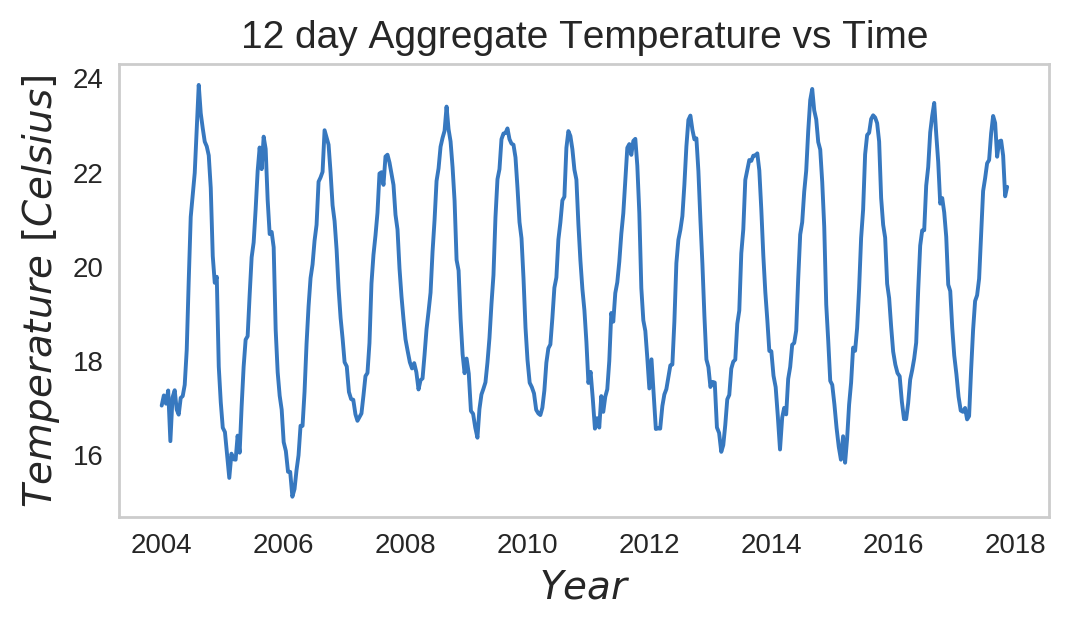
\includegraphics[width=1\linewidth]{ts.png}
\caption{\label{fig:ts}API includes a special time series generator for a selection.}
\end{minipage}
\end{figure}

Temperature data displayed in Figure~\ref{fig:ts} is modeled as a linear time series process using the theory described in Appendix~\ref{append:TS} after applying deseasonalizing the time series the methods described in Appendix~\ref{append:STL}.

Time series plotting capability is expanded two three dimensions as shown in Figure~\ref{fig:vts}. The first 100 meters water column is aggregated into ten equal partitions. Each partition is ten dbar/meters thick. Each aggregate has its time series, whose amplitude is described by color. 

\begin{figure}[H]
\centering
\begin{minipage}{4in}
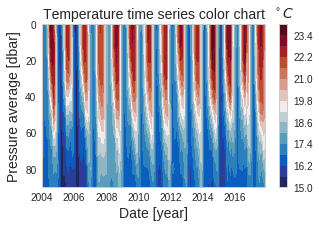
\includegraphics[width=1\linewidth]{tempColorChart.png}
\caption{\label{fig:vts}Time series at ten equally spaced partitions along the first 100 meters of the water column (10 meters/partition). Temperature is displayed as color and the y-axis is plotted as pressure (depth).}
\end{minipage}
\end{figure}

Without modeling the time series, the plotting feature shows upwelling patterns in the years 2005-2007. Colder water is brought closer to the surface as indicated by the dark blue color. Years 2007 and 2008 show upwelling patterns; the color is much brighter than the surrounding years. Another item worth mentioning is the large thermal mass forming in winter 2017/2018. Arvovis's API can monitor this warm mass evolve daily being as the app updates its database daily.

Another method generates interpolated maps, again by aggregating the data, but only for one time range, shown by Figure~\ref{fig:contourPlotSelection}.
The histogram summarizes the temperature distribution over the whole time series in Figure~\ref{fig:tempHist}.

\begin{figure}[H]
\centering
\begin{minipage}{4in}
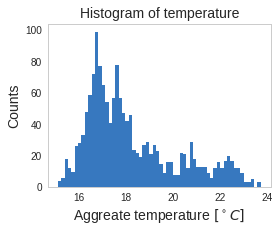
\includegraphics[width=1\linewidth]{tempHist.png}
\caption{\label{fig:tempHist}Histogram of temperatures of the first 100 dbar/meters, aggreagated into 10 dbar sections.}
\end{minipage}
\end{figure}

The histogram shows a bivariate data set (most likely seasonal) with a right-hand skew (surface temperatures). Summary statistics are provided in Table~\ref{tbl:tempHist}.

\begin{table}[hbt]
\centering
\caption{Anomaly Distribution Properties \label{tbl:tempHist}}
{\begin{tabular}{|c|c|}
\hline
\textbf{Statistic} & \textbf{Value} $[^\circ C]$
\\ \hline
Mean\hphantom{00} & \hphantom{0}$18.2456$
\\ \hline
Median\hphantom{00} & \hphantom{0}$17.6627$
\\ \hline
Min\hphantom{00} & \hphantom{0}$15.0946$
\\ \hline
Max\hphantom{00} & \hphantom{0}$23.7158$
\\ \hline
Standard Deviation\hphantom{00} & \hphantom{0}$1.9496$
\\ \hline
Skew\hphantom{00} & $0.8933$
\\ \hline
Kurtosis (Pearson's) \hphantom{00} & $-0.1797$
\\ \hline
\end{tabular} }
\end{table}

\begin{figure}[H]
\centering
\begin{minipage}{4in}
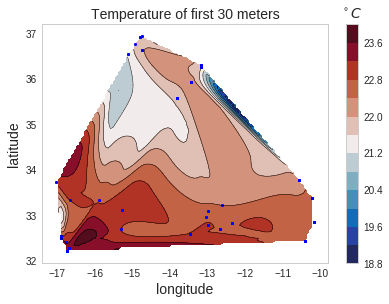
\includegraphics[width=1\linewidth]{contourPlotSelection.png}
\caption{\label{fig:contourPlotSelection}Cubic interpolation of temperature at the first 30 meters of arbitrary selection.}
\end{minipage}
\end{figure}

The API also has a built-in histogram on a map, showing profile frequency on a $1\times 1$ degree grid, shown by Figure~\ref{fig:worldHist}.

\begin{figure}[H]
\centering
\begin{minipage}{6in}
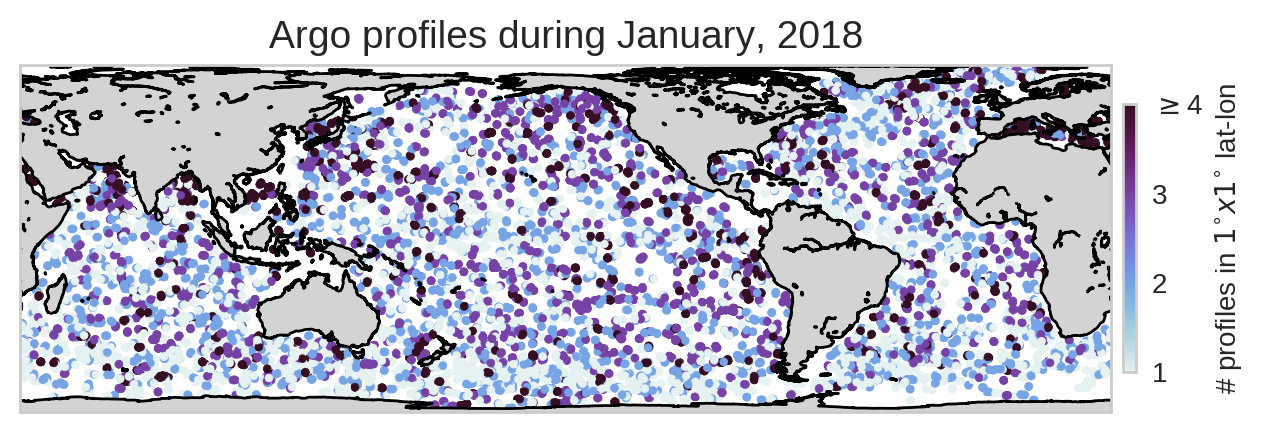
\includegraphics[width=1\linewidth]{worldHist.png}
\caption{\label{fig:worldHist}Frequency of profiles in a $1\times 1$ degree grid during January 2018.}
\end{minipage}
\end{figure}

\section{Conclusion}

Argovis has proved that it is feasible to implement modern web-app tools for scientific application. Web-apps with similar architecture can be used as interfaces for other large climate/oceanographic datasets. A map-based interface also allows gridded products generated from the Argo datasets can be displayed side-by-side for comparison. As Argovis grows in complexity, front-end frameworks such as Angular or React.js are used to separate client-side logic in a \gls{mvc} design. Rewriting the front end this way improves the maintainability of the app and expands the capability to handle more complex features all the while sustaining the cost of running and maintaining this app.

It is in the interest of international incentives such as Argo to have a broad user community. The Argo program depends on the public support to thrive. Apps that allow ordinary people visualize their tax dollars at work bolster their support. Argovis is intuitive enough for non-programmers to use. K-12 schools may use it in their in ocean science education. Argovis can be featured at ocean science centers, displayed on public kiosks. Learning to use the app requires little to no training other than basic 'point-and-click' computer proficiency, as shown by the tutorials shown earlier in this chapter. The openness of the app lets students, in turn, to show it to their friends and family. Data visualization tools already exist for Argo but are unsuitable for researchers to use. Argovis addresses this by allowing automation tools for professionals.

The RESTfull API portion allows scientists to interface with the app's database, otherwise, they will be forced to grab data using a browser. Automation through the API ensures scientists focus more time on the non-trivial inferencing they will be doing with the data. Temperature and salinity measurements are also needed by biologists, climate scientists who undoubtedly have their preferred tools and programming languages. The API is customizable, tailoring to the needs of Argo's diverse community. The base functions displayed in Appendix~\ref{append:python_api} shows just how simple 'hooking' up to Argovis can be. Nothing is stopping the community from writing these four functions in R, Matlab, Julia, et cetera. Data is extracted in JSON format and adjusted into the tabular format in a few lines of code.

In sum, through its utility and ease of use, Argovis becomes the face of the Argo project. 